\documentclass[12 pt]{article}
\usepackage{amsmath}
\usepackage{natbib}
\usepackage{graphicx}
\usepackage{subfig}
\usepackage{bm}
\usepackage{appendix}
\usepackage{authblk}
\usepackage{subfig}
\usepackage{float}
\usepackage{booktabs}

% edges & space between lines
\renewcommand{\baselinestretch}{1.65}
\renewcommand{\arraystretch}{.5}
\addtolength{\textwidth}{1.2in}
\addtolength{\oddsidemargin}{-.6in}
\addtolength{\evensidemargin}{-.8in}
\addtolength{\textheight}{0.5in} \addtolength{\topmargin}{-.2in}

% Special commands 
\newcommand{\vect}[1]{\boldsymbol{\mathbf{#1}}}
\providecommand{\e}[1]{\ensuremath{\times 10^{#1}}}

\title{Trade and Inequality in the Spatial Economy}
\author[1]{Farid Farrokhi}
\author[2]{David Jinkins\thanks{We thank Sina Smid for research assistance, and participants in seminars at Cardiff University, Copenhagen Business School, Copenhagen University, and Penn State for helpful suggestions.}}
\affil[1]{Penn State}
\affil[2]{Copenhagen Business School}
\renewcommand\Authands{ and }

\begin{document}
\maketitle

Inequality has long fascinated economists, and growing income inequality has been recently and heatedly discussed in public forums.\footnote{It is not every year that a 700-page collection of charts and academic theory on inequality is a New York Times bestseller.} A remarkable fact emerging from this discussion is the strong positive relationship between wage inequality and city size \citep{baum2012understanding}.  In this paper, we add to the study of inequality and distribution of economic activity in two ways. First, we document new facts on the interaction of geography with inequality. Second, we develop a quantifiable model which explains our findings and their implications. In particular, we study the effects of improving trade infrastructure on wage and welfare inequality.

Our first contribution is to document facts about inequality and geography.  We assign to each American city a measure of remoteness meant to capture its distance from all other cities.  We then show that this measure correlates negatively with the skill premium, the ratio of the mean wage of college degree to the mean wage of non-college degree workers. That is, wage inequality is lower in remote cities. On the other hand, the less remote a city is, the higher its share of college degree workers. To our knowledge, our paper is the first to document these two facts.

The literature has developed little in the way of a unified framework that incorporates both geography and inequality in the spatial economy. On one hand, economic geography examines the role of trade costs in determining spatial patterns of economic activity. This literature does not address inequality but welfare at the aggregate.  A classic example is \citep{krugman1991increasing}, and a more recent one is \citet{allen2014trade}. On the other hand, recent models of spatial inequality often treat cities as isolated. Workers in a city interact with each other but cities in a nation either do not trade or trade costlessly \citep{davis2014comparative}. Since the geographic location of a city relative to other cities remains irrelevant, this literature cannot address the interaction of geography with inequality. By including costly trade between cities in a model of mobile heterogeneous labor, we bridge the gap.

In our model, we have a continuum of locations, workers, and firms.  Workers come in two types, skilled and unskilled, and each worker has an ideosyncratic utility from living in each location.  A worker decides where to live taking wages as given.  A firm also takes local wages as given, and produces a tradable good using skilled and unskilled labor as inputs.  The sole difference between the two types of labor is that skilled labor benefits more from agglomeration.\footnote{We allow there to be a Hicks-neutral agglomeration force as well.}

We require a model which generates skill premia differing across locations.  In particular, to match our empirical findings we want less remote cities to have higher skill premia.  We develop a model with two critical features which delivers the required relationship.   The two critical features are stronger agglomeration forces for skilled workers, and heterogenous location preferences.

The intuition behind the model can be described in a few sentences.  Consider a city near other cities, a centrally-located city.  Its access to cheap tradable goods and nearby markets make it attractive to live in.  This leads the city, all else equal, to have a relatively high population compared with a remote city.  Due to agglomeration forces, skilled workers become relatively more productive in the centrally-located city.  Thus, all else equal, firms there demand a relatively high share of skilled workers as inputs.  In order for the relative share of skilled workers on the supply side to equal the firm's demand for relative share of skilled workers as inputs, there must be a higher skill premium in the centrally-located city.

Simulation results show that improving trade infrastructure benefits both types of labor, but low skill labor benefits more.  Better infrastructure tends to spread populations out, so that skilled workers lose some of their agglomeration advantage over unskilled workers.  Typically models of inequality and trade predict that skilled workers gain more than unskilled workers \citep{antras2006offshoring}, a result that is reversed in our model.

The literature on the skill premium has found a number of patterns.  To the extent that we are able to measure the relevant variables, all of these facts are consistent with our data.  The literature has shown convincingly that the skill premium is higher in cities with larger populations \citep{davis2012spatial}.  The relationship between the skill premium and city size has become stronger over time \citep{baum2013inequality, lindley2014spatial}.  In addition, larger cities have been shown to have a higher share of college-educated worker, another pattern which has strengthened over time \citep{moretti2008real, lindley2014spatial}.  Areas of denser economic activity have higher skill premiums \citep{combes2012sorting}.

These stylized facts have inspired a number of theories \citep{davis2012spatial,davis2014comparative,baum2012understanding,combes2012sorting}.  These theories abstract from costly trade, treating trade between cities as either non-existant or frictionless.\footnote{\citet{davis2012spatial} does contain an extension where trade costs are treated in the limit as they go to zero.}  The style of our modeling exercise below has more in common with recent forays of trade economists into economic geography \citep{allen2014trade,desmet2014geography,fajgelbaum2015state}.  These theories model costly trade, and focus on the spatial location of economic activity. They have, however, only one type of labor, so they cannot analyze the interaction between geography and inequality.  In an international trade context, \citet{fujita2006globalization} study inequality with costly trade, but their model has immobile unskilled workers.

A recent working paper, \citet{fan2015internal} analyzes the impact of an international trade liberalization on inequality using a spatial equilibrium framework.  As Fan's focus is on aggregate welfare effects rather than on the forces determining the distribution of the skill premium, he relies on skilled and unskilled workers differentially valuing amenities to generate the observed distribution of the skill premium.\footnote{Skilled and unskilled workers in \citet{fan2015internal} differ in terms of valuation of amenities, draws from productivity distributions, costs of migration, and initial allocations across space.  The initial allocations are important as migration costs depend on the location a worker starts from.}  Since we are interested in the geographic distribution of inequality, we have a much simpler model in which skilled workers only differ from the unskilled in terms of strength of agglomeration effects in the production function.

\section{Documenting inequality and geography}

In this section, we describe our data sources, give our definitions of measures of geography and inequality, and present the empirical findings which motivate our modeling exercise.

\subsection{Data sources}

Our empirical section is based on data from the 2000 American census public use micro-data (IPUMS) 5\% sample.\footnote{We clean the data using modified replication code from \citet{baum2013inequality}, which is available on Nathanial Baum-Snow's website.}  In this cut of the data, we use individuals older than 24 and younger than 65 with reported income, giving us observations on over four million workers distributed across the United States.

We want to compare inequality in different locations.  For our purposes, a location will be a US county.  There are more than 3000 counties in the United States.  In order to think about the geography of counties, we need to know the precise location of each county in space.  We download a population weighted centroid for each county from the Missouri census data center (http://mcdc2.missouri.edu/websas/geocorr2k.html).


\subsection{Important concepts}

Our main measure of geography is remoteness, a concept we borrow from the international trade literature.\footnote{It is a famous empirical regularity that the trade of two countries is proportional to the product of their national products divided by the physical distance between them.  This relationship is known as the naive gravity equation.  The adjective naive makes an appearance because such a gravity equation implies that trade between two countries is unaffected by what takes place in a third country.  For example, the trade between the United States and Mexico is unaffected by the rapid increase in trade between China and the United States.  Remoteness in an international trade context is the national-product-weighted sum of the distance between a country and all other countries.  Multiplying the gravity equation by a remoteness term allows third countries to influence bilateral trade relationships.}  The particular functional form we use is based on a suggestion in \citet{head2003gravity}.  We label each county with a number $i=1\dots N$.  The population of county $i$ is $P_i$, and the geodesic distance, i.e. the distance as the crow flies, between county $i$ and county $j$ is $d_{i,j}$.  The remoteness of county $i$ $R_i$ is given by:

\begin{equation}
    R_i = \frac{1}{\sum_{j\neq i} \frac{P_j}{d_{i,j}}} \nonumber
    \label{eq:rem}
\end{equation}

In words, an county which is close to other counties with high populations will have low remoteness.  We want this measure to reflect the ease with which a location can trade with other locations.  This measure does not, of course, take into account geographic features such as rivers, mountains, roads, and airports, but physical distance is still an important part of transportation cost.

We have two measures of inequality, the college wage premium (or skill premium) and the college population share (or skill share).  Both are measured in a way standard in the labor literature, and are calculated in each county.  A worker is highly educated if he has a four-year college degree.  The college premium is the mean wage of highly-educated workers in a county divided by the mean wage of other workers.  The college population share is the population of highly-educated workers in a county divided by the population of less-educated workers.  When calculating all means, we use census population weights.

Table \ref{tab:sum_stats} contains some descriptive statistics.  Figure \ref{fig:geo} shows how our measures vary across the United States. In each of these figures, the blue background is remoteness, with deeper blues signifying higher remoteness.  Remoteness has an obvious geographic pattern, lowest on the Northern East and Southern West Coasts.   Dark dots in the other figures signify counties with the highest levels of the variable listed under the figure.  The college wage premium is higher on the East Coast and in the South than it is in the Midwest and the Pacific Northwest.  College share follows a similar pattern.

\begin{table}[H]
    \centering
    \begin{tabular}{lll}
        \midrule
        Statistic           & Mean      & Standard Dev \\
        \midrule
        Remoteness          & 2.4\e{-6} & 1.1\e{-6} \\
        Population          & 2.3\e{5}  & 5.3\e{5}  \\
        Skill premium       & 1.58      & 0.15      \\
        College share       & 0.37      & 0.26      \\
        \midrule
        Census observations & 4.3\e{6}  & \\
        County observations & 815       & \\
        \midrule
    \end{tabular}
    \caption{Data summary statistics}
    \label{tab:sum_stats}
\end{table}

\begin{figure}[!ht]
  \centering
  \subfloat[Remoteness]{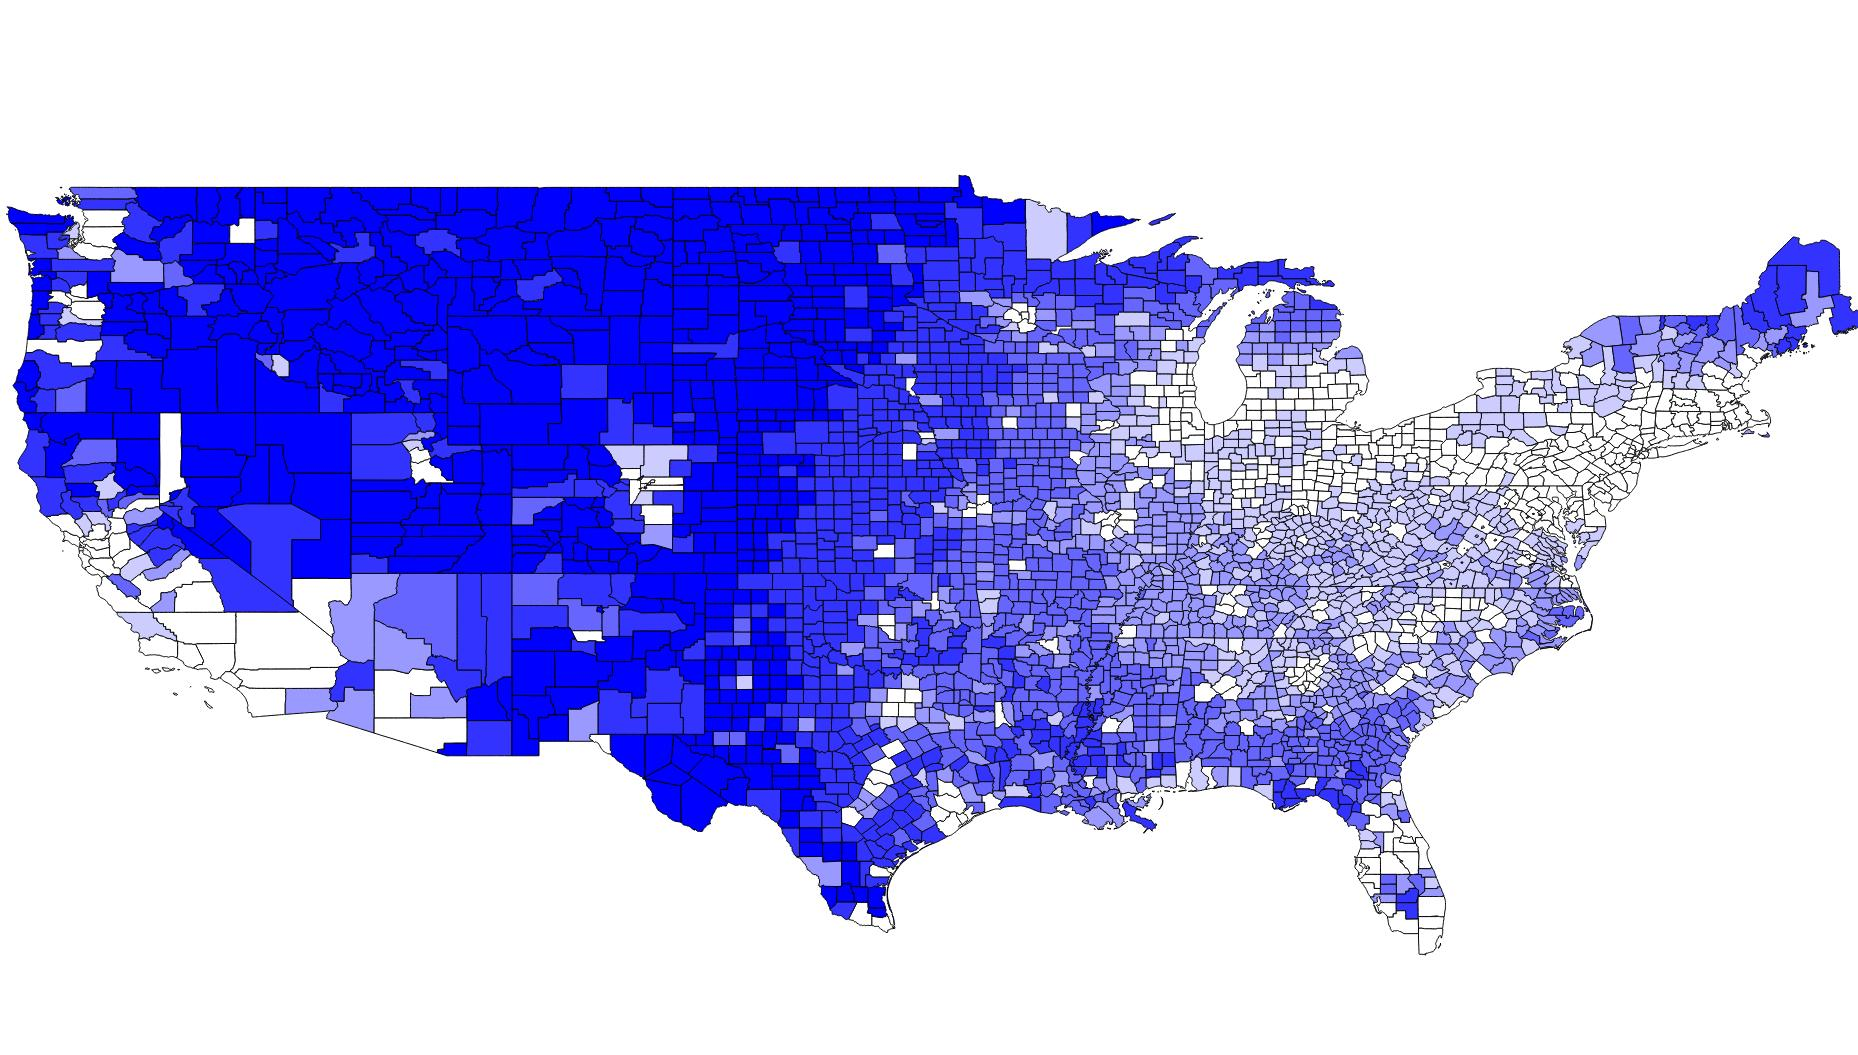
\includegraphics[width=.5\textwidth]{pics/rem.jpeg}}\quad
  \subfloat[Population]{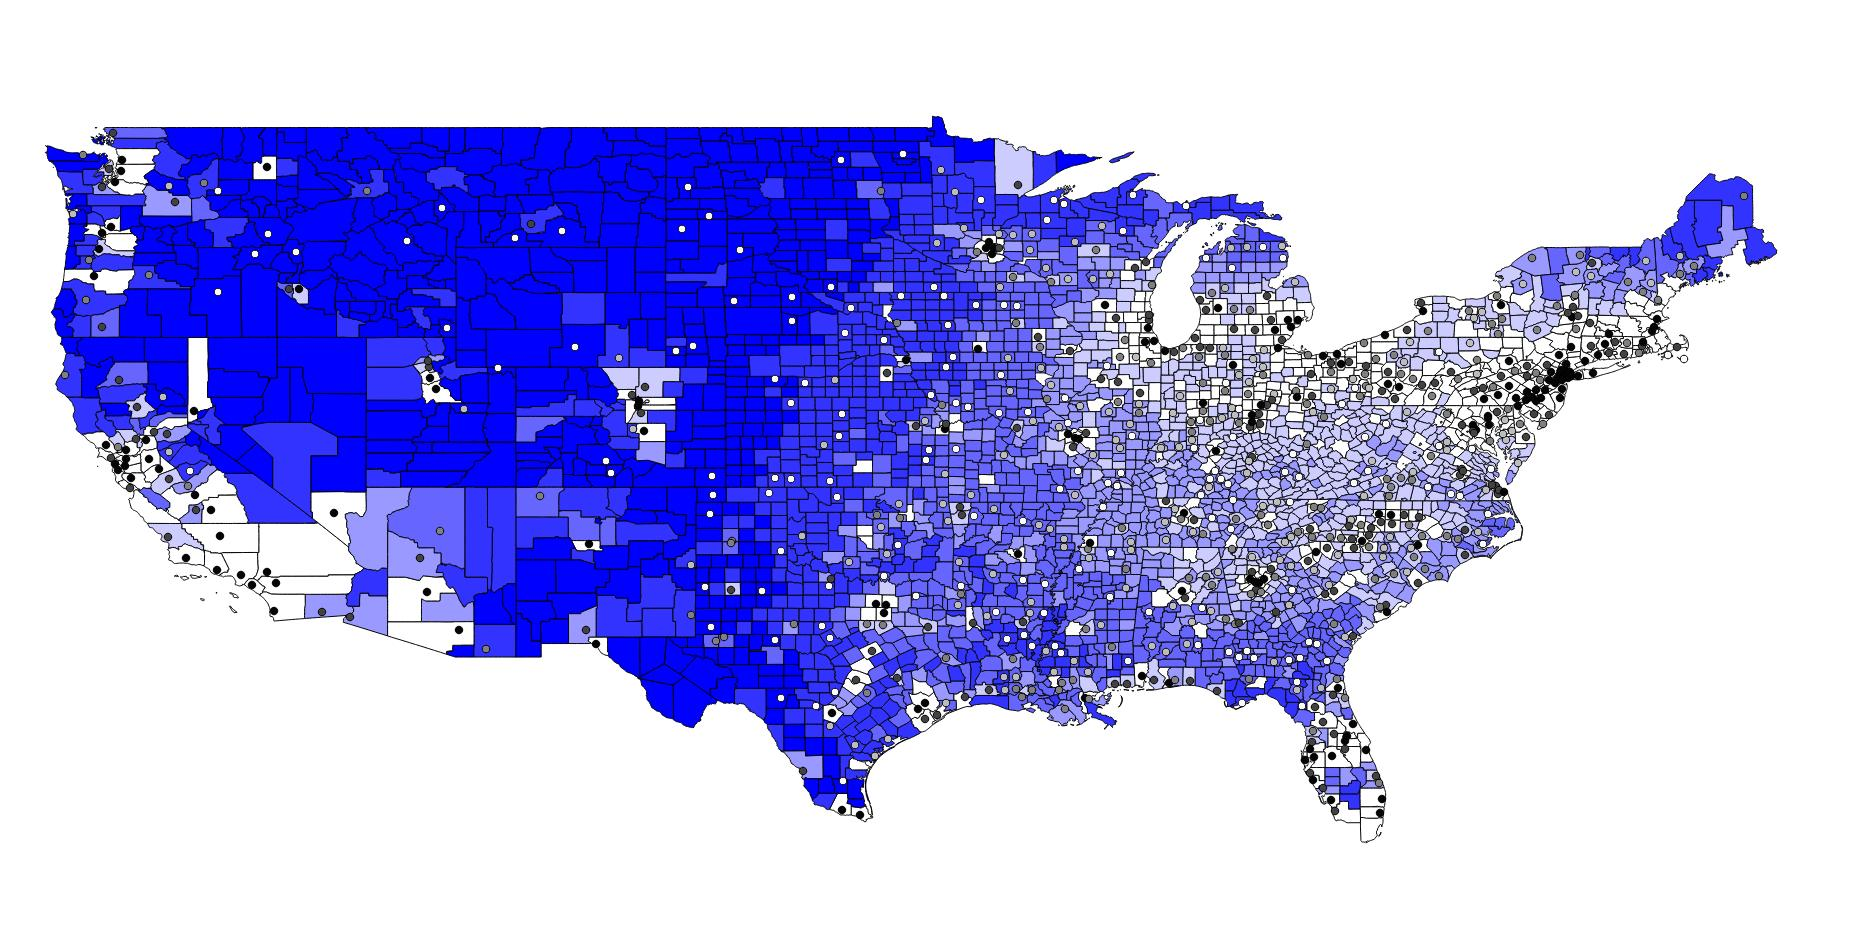
\includegraphics[width=.5\textwidth]{pics/pop.jpeg}}\\
  \subfloat[Skill Premium]{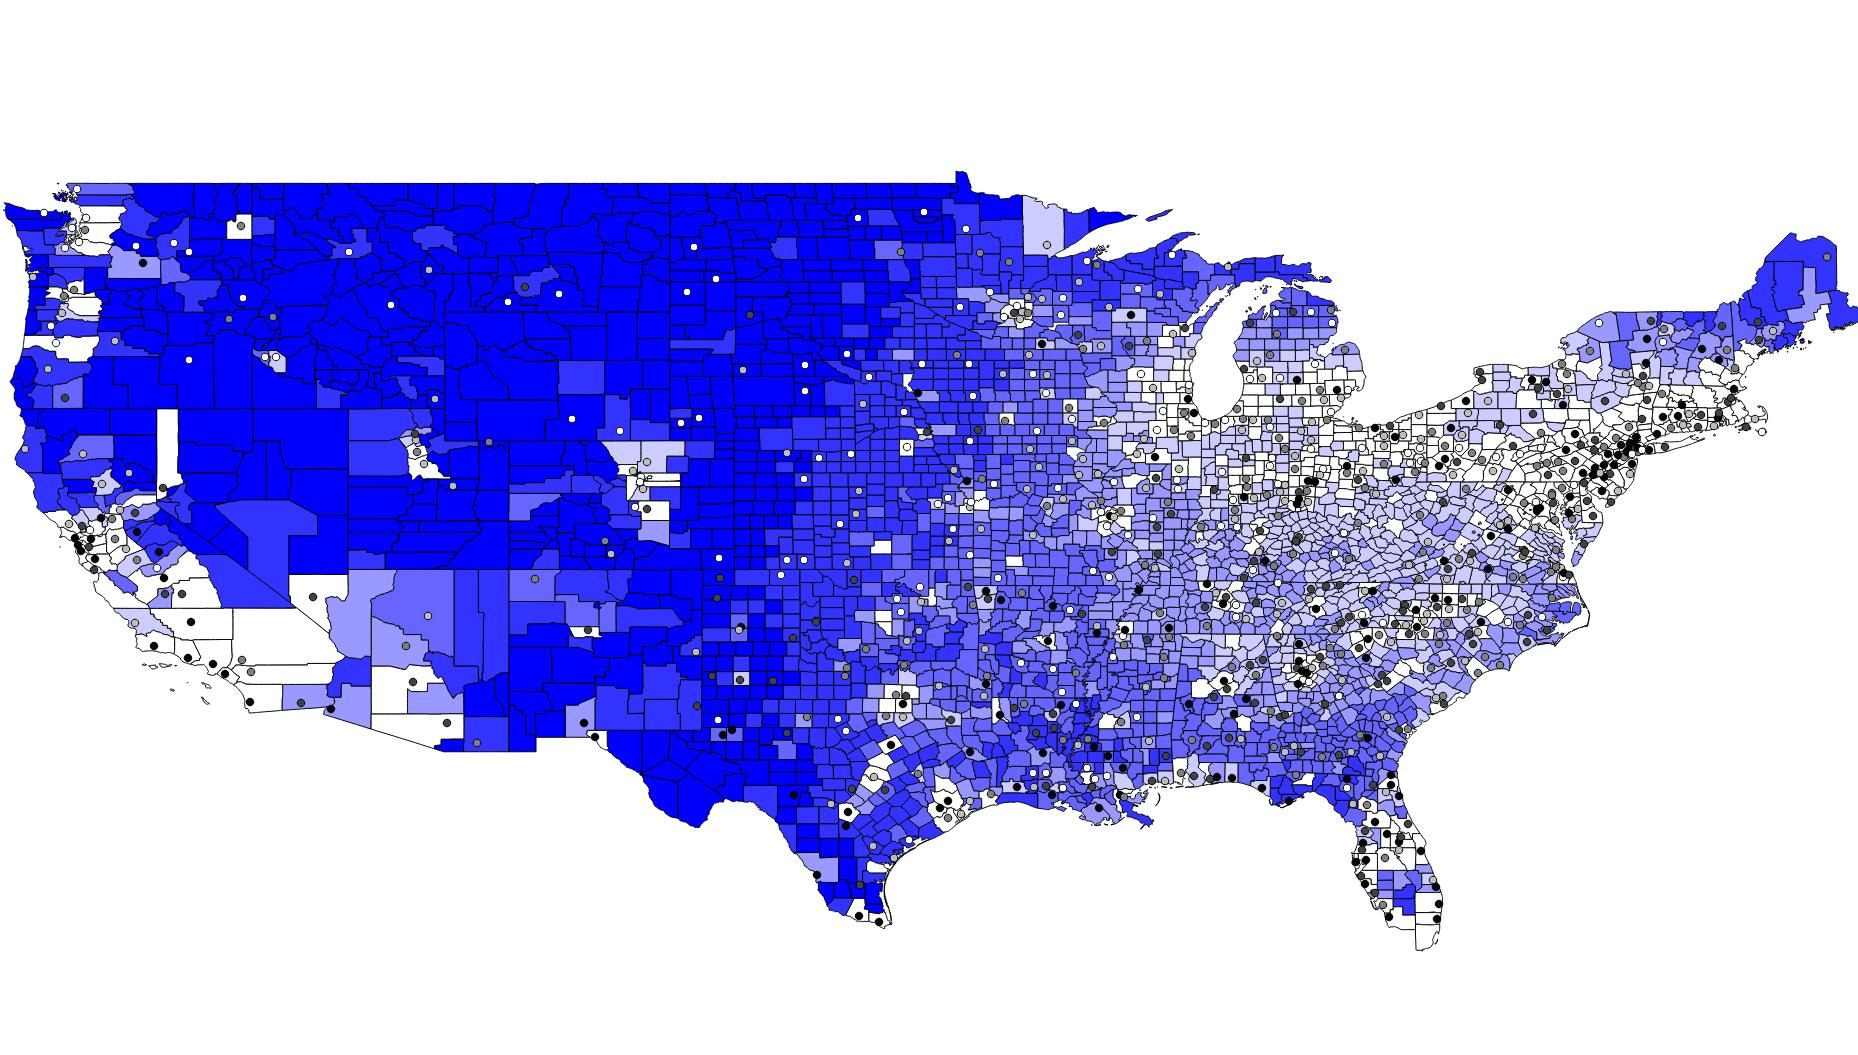
\includegraphics[width=.5\textwidth]{pics/college_wage_premium_alt.jpeg}}\quad
  \subfloat[College Share]{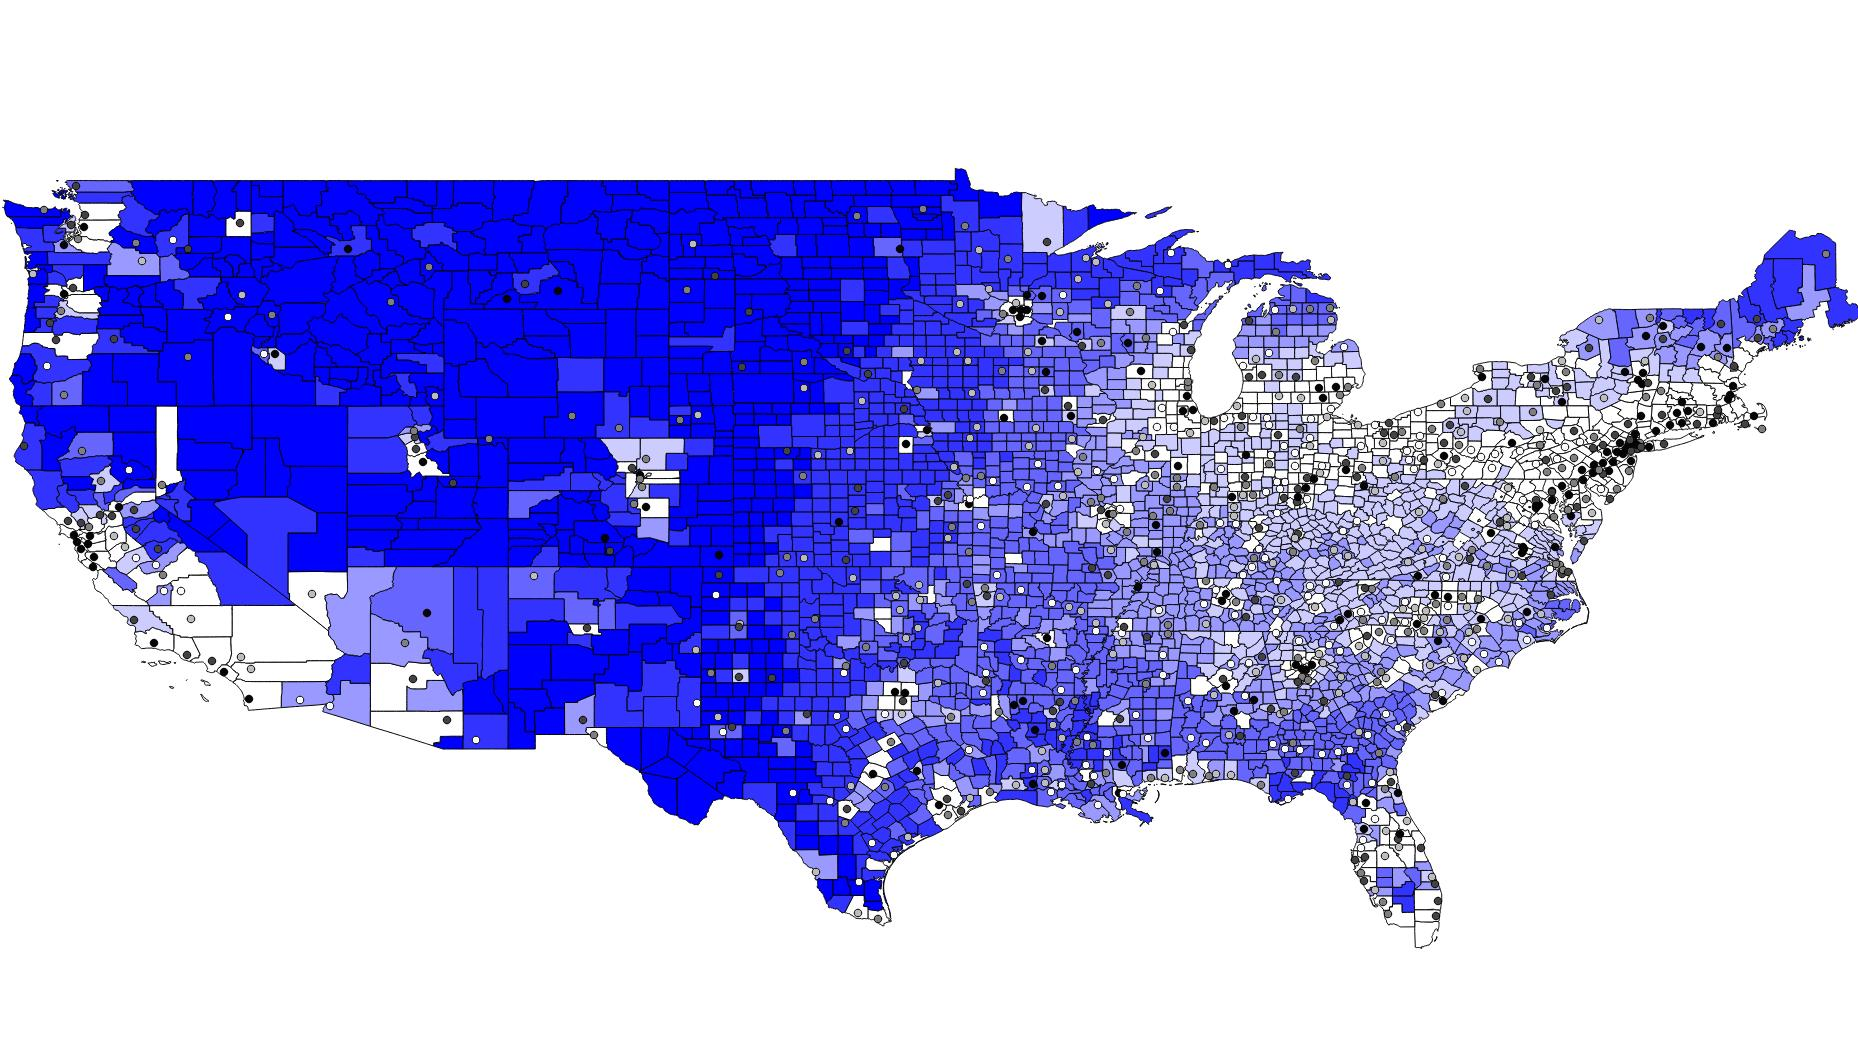
\includegraphics[width=.5\textwidth]{pics/college_pop_ratio.jpeg}}
  \caption{Counties by data feature}
  \label{fig:geo}
\end{figure}

\subsection{Empirical results}
In this section we document the covariance of our measure of geography, remoteness, with our measures of inequality, the college wage premium and college share.  Regressions of the skill premium on remoteness and other variables are found in Table \ref{tab:skill_reg}.  Remoteness covaries negatively with the skill premium, with an elasticity of 5\%.  We find that the population of a county varies positively with the skill premium, a result that has been emphasized in other studies.  That the coefficient on population loses significance with state fixed effects is a provocative result.  The covariance of remoteness and the skill premium is in the opposite direction and significant in all specifications.

In Table \ref{tab:col_reg} we report coefficient estimates from regressions of college population share on the same regressors.  We find that remoteness covaries positively with the college population ratio.  Nearly everything said about the was before, the magnitude of the population effect and the remoteness effect are similar.  The one difference is the population remains significant after including state fixed effects.

The takeaway from the empirical section is that we have identified a new relationship in the data.  Relatively remote counties in the United States have relatively low college wage premia, and relatively low college population shares.  As has been found in the previous literature we find that relatively high population counties also have relatively high college wage premia and relatively high college population shares.  These two facts motivate the theory developed in the next section.

% This table was done using estout package in stata, which is why the code looks so ugly!
\begin{table}
    \centering
    \begin{tabular}{lccc} \hline
     & (1) & (2) & (3) \\
    VARIABLES & log wage prem & log wage prem & log wage prem \\ \hline
    \vspace{4pt} & \begin{footnotesize}\end{footnotesize} & \begin{footnotesize}\end{footnotesize} & \begin{footnotesize}\end{footnotesize} \\
    log remoteness & -0.0562*** & -0.0367*** & -0.0310** \\
    \vspace{4pt} & \begin{footnotesize}(0.00558)\end{footnotesize} & \begin{footnotesize}(0.0113)\end{footnotesize} & \begin{footnotesize}(0.0125)\end{footnotesize} \\
    log population &  & 0.00809** & 0.00432 \\
    \vspace{4pt} & \begin{footnotesize}\end{footnotesize} & \begin{footnotesize}(0.00391)\end{footnotesize} & \begin{footnotesize}(0.00431)\end{footnotesize} \\
    constant & -0.275*** & -0.113 & 0.0495 \\
     & \begin{footnotesize}(0.0728)\end{footnotesize} & \begin{footnotesize}(0.112)\end{footnotesize} & \begin{footnotesize}(0.123)\end{footnotesize} \\
    \vspace{4pt} & \begin{footnotesize}\end{footnotesize} & \begin{footnotesize}\end{footnotesize} & \begin{footnotesize}\end{footnotesize} \\
    State FE & \mbox{no} & \mbox{no} & \mbox{yes} \\
    Observations & 815 & 815 & 815 \\
     $R^2$ & 0.119 & 0.124 & 0.307 \\ \hline
    \multicolumn{4}{c}{\begin{footnotesize} Robust standard errors in parentheses\end{footnotesize}} \\
    \multicolumn{4}{c}{\begin{footnotesize} *** p$<$0.01, ** p$<$0.05, * p$<$0.1\end{footnotesize}} \\
    \end{tabular}
    \caption{Regressions of log college premium on log geography variables}
    \label{tab:skill_reg}
\end{table}


% This table was done using estout package in stata, which is why the code looks so ugly!
\begin{table}
    \centering
    \begin{tabular}{lccc} \hline
     & (1) & (2) & (3) \\
    VARIABLES & log col share & log col share & log col share \\ \hline
    \vspace{4pt} & \begin{footnotesize}\end{footnotesize} & \begin{footnotesize}\end{footnotesize} & \begin{footnotesize}\end{footnotesize} \\
    log remoteness & -0.348*** & -0.182*** & -0.287*** \\
    \vspace{4pt} & \begin{footnotesize}(0.0288)\end{footnotesize} & \begin{footnotesize}(0.0536)\end{footnotesize} & \begin{footnotesize}(0.0682)\end{footnotesize} \\
    log population &  & 0.0692*** & 0.0485** \\
    \vspace{4pt} & \begin{footnotesize}\end{footnotesize} & \begin{footnotesize}(0.0190)\end{footnotesize} & \begin{footnotesize}(0.0236)\end{footnotesize} \\
    constant & -5.701*** & -4.312*** & -5.489*** \\
     & \begin{footnotesize}(0.375)\end{footnotesize} & \begin{footnotesize}(0.529)\end{footnotesize} & \begin{footnotesize}(0.675)\end{footnotesize} \\
    \vspace{4pt} & \begin{footnotesize}\end{footnotesize} & \begin{footnotesize}\end{footnotesize} & \begin{footnotesize}\end{footnotesize} \\
    State FE & \mbox{no} & \mbox{no} & \mbox{yes} \\
    Observations & 815 & 815 & 815 \\
     $R^2$ & 0.151 & 0.163 & 0.314 \\ \hline
    \multicolumn{4}{c}{\begin{footnotesize} Robust standard errors in parentheses\end{footnotesize}} \\
    \multicolumn{4}{c}{\begin{footnotesize} *** p$<$0.01, ** p$<$0.05, * p$<$0.1\end{footnotesize}} \\
    \end{tabular}
   \caption{Regressions of log college share on log geography variables}
    \label{tab:col_reg}
\end{table}

\section{Theory}
In the last section, we presented evidence that geography plays a role in shaping the college wage premia and college population shares. In this section we generalize spatial models of trade to explain our new finding as well as the previously documented facts. In particular, the model introduces a mechanism to explain why the college wage premium and college population share both decrease with the remoteness of a location.

\subsection{Environment}

The model is static, with a continuum of locations $j \in J$, a continuum of skilled workers with total population $N_H$, and a continuum of unskilled workers with total population $N_L$.  Workers can choose to reside and work in any (single) location.  Firms in each location can produce a location-specific variety of a tradable final good with a constant elasticity production function using the two types of labor as inputs. Both workers and firms are price takers in perfectly competitive markets.

\subsection{Worker's problem}

The utility of a worker in location $i$ is:
\begin{eqnarray}\label{eq:utility}
	Q(i) u(i) \epsilon(i)
\end{eqnarray} 
where $Q(i)$ is utility from tradeables, $u(i)$ is the utility from exogenous amenities, and $\epsilon(i)$ is worker-specific preference for location $i$.  Tradeable goods are differentiated by the origin of production, and $q(j,i)$ is consumer's consumption in $i$ from goods originated in location $j$. The aggregator $Q(i)$ in the utility function with elasticity of substitution $\sigma>0$ is:
\[
	Q(i) = \left[\int_J q(j,i)^{\frac{ \sigma - 1}{\sigma}}~ dj\right]^{\frac{\sigma}{\sigma-1}},
\]
We assume that worker location prefrences $\epsilon(i)$ are independent across workers and locations, and have a Type II Extreme Value distribution,
\[
    \Pr(\epsilon(i) \leq x) = \exp(-x^{-\theta})
\]
Workers are endowed with exogenous skill $s \in \{H,L\}$. A worker's wage in location $i$ is denoted by $w_s(i)$, and her budget constraint is 
\begin{eqnarray}\label{eq:budget}
	w_s(i) = \int_J p(j,i)q(j,i)~dj 
\end{eqnarray}
where $p(j,i)$ is price of good $j$ in destination $i$, and $J$ is the given set of locations.  The \emph{only} place skill type appears in the worker's problem, is through the wage's effect on the budget constraint.  Otherwise workers of both types have the same preferences.

A worker has two types of decision to make.  She decides where to live, and how much of each good to consume.  Given a choice of location, the second problem is standard.  A worker of type $s$ in location $i$ spends $x_s(j,i)$ on goods produced in $j$,
\begin{eqnarray}\label{eq:x_s}
	x_s(j,i) & \equiv & p(j,i) q_s(j,i) = \Big[ \frac{p(j,i)}{P(i)} \Big]^{1-\sigma} w_s
\end{eqnarray}
where $P(i)$ is the CES price index,
\begin{eqnarray}\label{eq:price_index}
	P(i) = \left[\int_J p(j,i)^{1-\sigma}~ dj\right]^{\frac{1}{1-\sigma}}
\end{eqnarray}

The second decision a worker makes is where to live.  In order to characterize this decision, we introduce congestion forces as in \citet{allen2014trade}:
\begin{eqnarray}\label{eq:congestion}
u(i) = \bar{u}(i)  n(i)^{\gamma}
\end{eqnarray}
Here, $n(i)$ is total population in location $i$ and $\gamma<0$ is the degree of congestion effect. This specification is isomorphic to a setting where preferences are Cobb-Douglas between tradeables and housing in which housing supply is inelastic.
A worker with skill level $s$ faces the following discrete choice problem over locations:
\begin{eqnarray} 
\max_{i \in J}~ \frac{w_s(i)}{P(i)}u(i) \epsilon(i)  \nonumber
\end{eqnarray}
Using the properties of the Type-II extreme value distribution, we can characterize the share of type-$s$ labor in location $i$ as:\footnote{Incidentally this equation gives the model its first testable prediction:
    \begin{equation*}
        \frac{\frac{w_H(i)}{w_L(i)}}{\frac{n_H(i)}{n_L(i)}^\frac{1}{\theta}} = \frac{\frac{w_H(j)}{w_L(j)}}{\frac{n_H(j)}{n_L(j)}^\frac{1}{\theta}}
    \end{equation*}
    A higher ratio of skilled workers to unskilled workers implies a higher skill premium in wages.  In the data, the college wage premium and college population share are strongly positively correlated.  A simple regression implies a $\theta$ value of $1.5$.}

\begin{eqnarray}
    \frac{n_s(i)}{n_s(j)} = \left(
	\frac{w_s(i)u(i)/P(i)}
	{w_s(j)u(j) /P(j)}\right)^\theta
    \label{eq:rel_pops}
\end{eqnarray} 
where $n_s(i)$ is population of workers with type $s$ in location $i$.
The elasticity of relative labor supply to relative wages is:
\[
\frac{ \partial \Big(n_s(i)/n_s(j)\Big) \Big/
\Big(n_s(i)/n_s(j)\Big)}
{\partial \Big(w_s(i)/w_s(j)\Big) \Big/
\Big(w_s(i)/w_s(j)\Big) } = \theta
\]
The variance of $\epsilon(i)$ across both workers and locations is decreasing in $\theta$. A large $\theta$ implies that individual unobserved preferences for location are similar across locations. Small changes in wages, prices, or amenities induce large movements of workers.  Another way of putting it is that the supply curve of workers to a location is flat.  When $\theta$ is small, workers have widely varying preferences over locations, so that large changes in wages, prices, or amenities are necessary to induce movement.  That is, the supply curve of workers to a location is steep.

A location with a higher relative wage for skilled workers will attract relatively more skilled workers, but it won't attract all the skilled workers.  Small changes in relative wages will induce small changes in relative populations.  In a model without preference heterogeneity, in equilibrium all populated locations must offer the same utility within skill type.  This means that a location which deviates and offers a slightly higher wage will attract \emph{all} workers.

Define the well-being index, denoted by $W_s$, for population of skill $s$:
\begin{equation*}
    W_s \equiv \left[\int_{j=0}^{\|J\|}\left(w_s(j) P(j)^{-1} u(j)\right)^\theta dj\right]^{\frac{1}{\theta}}
\end{equation*}
This index is proportional to the expected welfare of a worker of type $s$ before she draws her location preferences.\footnote{To get the actual welfare, we must multiply by the gamma function $\Gamma(1 +\frac{1}{\theta})$.  This scaling term depends only upon $\theta$, an exogenous preference parameter.}  Again using properties of the Type-II extreme value distribution, we derive the relationship for all $i \in J$:
\begin{eqnarray}\label{eq:indiff}
    \frac{n_s(i)}{N_s} = \left(\frac{w_s(i) P(i)^{-1} u(i)}{W_s}\right)^{\theta}
\end{eqnarray}
Here $N_s$ is the exogenously given total population of type-$s$ workers. If a location offers relatively high welfare, it will have a relatively high population, with the extent of the relationship governed by $\theta$.

\subsection{Firm's problem}
Each location has a representative firm with a CES production function using skilled and unskilled workers,
\begin{eqnarray}
	 A(i)\Big[ \beta_H(i) n_H(i)^{\frac{\psi-1}{\psi}} + \beta_L(i) n_L(i)^{\frac{\psi-1}{\psi}} \Big]^{\frac{\psi}{\psi-1}} \nonumber
\end{eqnarray}
where $A(i)$ is total factor productivity in location $i$. $\psi>0$ is the elasticity of substitution between high and low skill workers. $\beta_H(i)>0$ and $\beta_L(i)>0$ are factor intensities. Differences in factor productivities (and agglomeration, to be discussed shortly) are the \textit{only} differences between skilled and unskilled labor. 
Following the literature, we distinguish two agglomeration forces. First 
\begin{eqnarray}\label{eq:agglom_general}
A(i) = \bar{A}(i) n(i)^{\alpha}
\end{eqnarray}
with $\alpha>0$. This agglomeration force changes productivity of both low and high skill workers. A standard Krugman type monopolistic competition with free entry generates the same relation through endogenous measure of firms (if $\alpha=1/(1+\sigma)$). In addition, there is strong evidence that agglomeration forces are stronger for high skill workers \citep{glaeser2010complementarity}.  Motivated by these findings, we make a skilled worker's productivity covary positively with the population of skilled workers in a city:
\begin{eqnarray}\label{eq:agglom_specific}
	\beta_H(i) & = & \bar{\beta}_H(i) n_H(i)^{\varphi} \nonumber \\
	\beta_L(i) & = & \bar{\beta}_L(i)
\end{eqnarray}
Here, $\varphi>0$ governs the skilled bias technological change for high skilled labor.
By cost minimization, the unit cost of production equals
\begin{eqnarray}\label{eq:unit_cost}
    \frac{c(i)}{A(i)} ,~\mbox{where}~~c(i)=\Big[ \beta_H(i)^{\psi} w_H(i)^{1-\psi} + \beta_L(i)^{\psi} w_L(i)^{1-\psi}\Big]^{\frac{1}{1-\psi}}
\end{eqnarray}
The share of spending of producers on high skill workers, denoted by $b(i)$, is given by
\begin{eqnarray}\label{eq:input_share}
	b(i) = \frac{\beta_H(i)^{\psi} w_H(i)^{1-\psi}}{\beta_H(i)^{\psi} w_H(i)^{1-\psi} + \beta_L(i)^{\psi} w_L(i)^{1-\psi}}
\end{eqnarray}
As $\beta_H(i)$ is increasing in the population of skilled workers in a city, so is $b(i)$.

Now the intuition for our result is available.  Suppose a new highway is built to a city. As a result of reductions in trade costs, the city will benefit from a lower price index and higher sales abroad, so firms in the city will attract workers of both types.  As the city grows, productivity rises. However, due to agglomoreation advantages, skilled workers become relatively more productive.  Firms will demand relatively more skilled workers.  There will be a disequilibrium as firms demand relatively more skilled workers than the skill share in the population.  Equilibrium is restored by raising skilled wages, which will both attract skilled workers and discourage firms from hiring them.

As mentioned above, markets are perfectly competitive. Let $d(j,i)$ be the trade costs of shipping a good from $j$ to $i$. The price of a good produced in location $j$ and consumed in location $i$ is $p(j,i) = c(j)d(j,i)/A(j)$. 

\subsection{Spatial Equilibrium}

A \textit{spatial equilibrium} is a set of $w_H(i)$, $w_L(i)$, $n_H(i)$, and $n_L(i)$ such that:\footnote{There is a bit hidden in this definition, as we have already used perfect competition to give us goods prices $p(j,i)$ given wages, the consumer's optimization problem to give us demand $x(j,i)$ given prices and wages, and the firm's optimization problem to give us relative labor demand \eqref{eq:input_share}}
\begin{enumerate}
\item Labor shares in locations are according to (\ref{eq:indiff}).
\item Demand and supply of skilled and unskilled labor are equal in each location.
\item Goods market clear
\begin{eqnarray}\label{eq:goods_mkt_clear}
	w_H(i) n_H(i) =  b(i) \int_J \sum_{s \in \{H,L\}} n_s(i)x_s(j,i) ~dj 
\end{eqnarray}
where $x_s(j,i)$ is given by (\ref{eq:x_s}), and $b(i)$ is given by (\ref{eq:input_share}).
\item Allocation of labor is feasible, $\int_J n_H(j) ~dj = N_H$ and $\int_J n_L(j) ~dj = N_L$. Wages are normalized $\int_J w_H(j) dj =1$.
\end{enumerate}

\vspace{5mm}
\subsection{Equilibrium Analysis}

Before we derive a system of equations characterizing the equilibrium, we first discuss some of its features.  In particular, we show that without both heterogeneous location preferences and skill-specific agglomeration, our model would not generate location-specific skill premia.  However, we need no other type of skill-specific preferences, productivity, or mobility to generate this result.

Perfect competition gives us that the income share of skilled labor equals firm's optimal input share on skilled labor:
\begin{eqnarray}
\frac{w_H(i) n_H(i)}{w_H(i) n_H(i) + w_L(i) n_L(i)}  = \frac{\beta_H(i)^{\psi} w_H(i)^{1-\psi}}{\beta_H(i)^{\psi} w_H(i)^{1-\psi} + \beta_L(i)^{\psi} w_L(i)^{1-\psi}} \nonumber
\end{eqnarray}
With some algebra, and substituting from (\ref{eq:agglom_specific}), we get:
\begin{eqnarray}\label{eq:labor_demand}
    \frac{n_H(i)}{n_L(i)} = \left(\frac{\bar{\beta}_H(i)}{\bar{\beta}_L(i)}\right)^\psi \left(\frac{w_H(i)}{w_L(i)}\right)^{-\psi} n_H(i)^{\varphi \psi }
\end{eqnarray}

Using equation (\ref{eq:indiff}), the supply side of labor markets imply:\footnote{As far as we are aware, other models of inequality in the literature assume fundamental differences in preferences between skilled and unskilled workers.  To derive \eqref{eq:labor_supply} we are using the fact that skilled and unskilled workers value amenities in the same way, and that they face the same prices.}
\begin{eqnarray}\label{eq:labor_supply}
    \frac{n_H(i)}{n_L(i)} = \frac{N_H}{N_L} \left(\frac{W_H}{W_L} \right)^{-\theta}
    \left( \frac{w_H(i)}{w_L(i)}\right)^{\theta}
\end{eqnarray}
Labor markets clear when skill premia simultaneously satisfy the pairs of demand (\ref{eq:labor_demand}) and supply (\ref{eq:labor_supply}).  Combining, we get:
\begin{eqnarray}\label{eq:labor_demand_supply}
    \frac{w_H(i)}{w_L(i)} = \left(\frac{W_H}{W_L}\right)^{\frac{\theta}{\theta + \psi}}\left(\frac{N_H}{N_L}\right)^{\frac{-1}{\theta + \psi}} \left(\frac{\bar{\beta}_H(i)}{\bar{\beta}_L(i)}\right)^{\frac{\psi}{\theta + \psi}} n_H(i)^{\frac{\varphi \psi}{\theta + \psi}}
\end{eqnarray}
Suppose we were to shut down preference heterogeneity, $\theta \rightarrow \infty$.  From \eqref{eq:labor_demand_supply} we see that the skill premium will be constant across locations (and, surprise, proportional to ex-ante expected welfare).  On the other hand, suppose there is no agglomeration for skilled workers, $\varphi = 0$.  Then the skill premium can vary between destinations only due to exogenous differences in returns to skilled and unskilled labor.  In order to have equilibria with (endogenously) varying skill premia, we need \emph{both} $\theta$ to be finite and $\varphi >0$. In words, we need both variance in unobserved location preferences and the agglomeration force for skilled workers.  Large cities demand more skilled workers due to agglomeration, but when unobserved location preferences matter skilled workers do not fully arbitrage the a wage increase away. In this respect, our model departs from a standard Rosen-Roback (or Allen-Arkolakis) model by highlighting the interaction of agglomeration and the labor supply elasticity. 

Next we show that the distribution of workers across space has a real effect on welfare inequality.  Plugging equilibrium skill premium from (\ref{eq:labor_demand_supply}) into relative labor supply (\ref{eq:labor_supply}), distribution of low skilled labor can be written as a function of distribution of high skilled labor,
\begin{eqnarray}\label{eq:labor_demand_supply_2}
n_L(i) = \Big( \frac{\bar{\beta}_H(i)}{\bar{\beta}_L(i)} \Big)^{\frac{-\theta\psi}{\theta+\psi}} 
\Big( \frac{W_H}{W_L} \Big)^{\frac{\theta\psi}{\theta+\psi}}
\Big( \frac{N_H}{N_L} \Big)^{\frac{-\psi}{\theta+\psi}}
\Big( n_H(i) \Big)^{\frac{\theta(1-\psi\varphi)+\psi}{\theta+\psi}}
\end{eqnarray}
Define $\rho_H(i) = n_H(i)/N_H$ as the density of high skill labor. Equation (\ref{eq:labor_demand_supply_2}) and $ N_L = \int_J n_L(i)~di $ pin down the relative average well-being of skilled and unskilled workers, $W_H/W_L$, as a function of $\rho_H(i)$,
\begin{eqnarray}\label{eq:WHtoL}
\frac{W_H}{W_L} & = &
\underbrace{~~\Big(\frac{N_H}{N_L}\Big)^{-\frac{1}{\psi}}~~}_{\mbox{aggergate scarcity}} \times \underbrace{~~(N_H)^{\varphi}~~}_{\mbox{aggregate agglom.}} \times \nonumber \\
&  &
\underbrace{\Bigg[ \int_J \Big( \frac{\bar{\beta}_H(i)}{\bar{\beta}_L(i)} \Big)^{\frac{-\theta\psi}{\theta+\psi}} \Big( \rho_H(i) \Big)^{\frac{\theta(1-\varphi)+\psi}{\theta+\psi}}~di \Bigg]^{-\frac{\theta+\psi}{\theta\psi}}}_{\mbox{distributional effect}} 
\end{eqnarray}
Equation (\ref{eq:WHtoL}) decomposes the three forces behind real well-being inequality: 1) Aggregate scarcity of high skill labor, 2) Aggregate agglomeration advantage of high skill workers, 3) A weighted average of relative exogenous productivities in which weights are determined by the the distribution of the density of high skill labor. While the  first two behave at the aggregate, the third relates to the distribution of skills. 
In this sense, Equation (\ref{eq:WHtoL}) relates an index of real inequality at the national level to the distribution of high skill workers across cities within the nation.
\subsection{Equilibrium equations}

In this section we characterize our equilibrium with only two integral equations.  These integral equations will be the basis of our empirical exercise.  

By simply inverting the definition \eqref{eq:input_share} of input share $b(i)$, we get total income in $i$ equal to $\frac{1}{b(i)} w_H(i)n_H(i)$. Using the goods market clearing condition, equation (\ref{eq:goods_mkt_clear}), we derive: 
\begin{eqnarray}
	w_H(i) n_H(i) b(i)^{-1} = 
	\int_J \Big[ \frac{c(i) d(i,j)}{A(i) P(j)} \Big]^{1-\sigma} w_H(j) n_H(j) b(j)^{-1} ~dj \nonumber
\end{eqnarray}

Equations (\ref{eq:unit_cost}) and (\ref{eq:input_share}) further imply that 
\begin{eqnarray}\label{eq:ctilde}
	c(i) & = & \tilde{c}(i) w_H(i) \nonumber \\
    \mbox{where}~~~ \tilde{c}(i) & = & 
	\Big[\bar{\beta}_H(i) n_H(i)^{\varphi}\Big] ^{\frac{\psi}{1-\psi}} \Big[b(i)\Big]^{\frac{-1}{1-\psi}}
\end{eqnarray}
Replacing $c(i)$ with $\tilde{c}(i)$ in the above integral equation and also replacing the price index using (\ref{eq:indiff}), after some algebra we get:
\begin{eqnarray}\label{eq:system1}
	& & A(i)^{1-\sigma} \tilde{c}(i)^{\sigma-1} n_H(i)  w_H(i)^{\sigma}  b(i)^{-1}  \nonumber \\
	& & =  
    W_H^{1-\sigma} N_H^{\frac{\sigma-1}{\theta}}
    \int_J d(i,j)^{1-\sigma} u(j)^{\sigma-1} n_H(j)^{(\theta+1-\sigma)/\theta} w_H(j)^{\sigma} b(j)^{-1}  ~dj
\end{eqnarray}
Again substituting the price index from (\ref{eq:indiff}) and $\tilde{c}(i)$ into (\ref{eq:price_index}), we get another integral equation: 
\begin{eqnarray}\label{eq:system2}
 	& &  u(i)^{1-\sigma} n_H(i)^{(\sigma-1)/\theta} w_H(i)^{1-\sigma}  = \nonumber \\ 
 	& & 
    W_H^{1-\sigma} N_H^{\frac{\sigma-1}{\theta}}
 	\int_J  d(j,i)^{1-\sigma} A(j)^{\sigma-1}  \tilde{c}(j)^{1-\sigma} w_H(j)^{1-\sigma}
 	~ dj
\end{eqnarray}
Equations \ref{eq:system1}--\ref{eq:system2} give us two systems of integral equations. If $\varphi=0$ and $\theta=\infty$, the integral equations collapse to those in \citet{allen2014trade}. 

We can reduce our system further using a method from \citet{allen2014trade}.  If either of the systems of integral equation hold along with the following relation, both systems of integral equations must hold:
\begin{eqnarray}\label{eq:systems_relation}
	  b(i)^{-1}  A(i)^{1-\sigma} \tilde{c}(i)^{\sigma-1} n_H(i)  w_H(i)^{\sigma} = \lambda  u(i)^{1-\sigma} n_H(i)^{(\sigma-1)/\theta} w_H(i)^{1-\sigma}
\end{eqnarray}
where $\lambda > 0$ is some constant.  The solution algorithm developed below is based on successive iterations over  $n_H(i)$.

There are two ``endogenous'' variables hidden in \eqref{eq:system1} - \eqref{eq:systems_relation}, $b(i)$ and $\tilde{c}$. Endogenous here means that they depend upon $n_H(i)$.  Thus solving our model involves an inner loop to update these endogenous variables.  Details of our solution algorithm are contained in Appendix \ref{sec:sol_alg}.

\citet{allen2014trade} have a slick proof of uniqueness, which depends only on the relationship between parameters governing agglomeration and parameters governing congestion.  Unfortunately the same proof cannot be used in our setting.  Intuitively, there should be a similar condition in our model relating the agglomeration forces to the congestion force will be that the parameter governing joint agglomeration $\alpha$ and the parameter governing skilled agglomeration $\varphi$ cannot be too large relative to the parameter governing congestion $\gamma$.  

\section{Simulation}

We are currently in the process of estimating the model, but the results are not ready yet.  At the moment, we present a simulation of the model, calibrated to replicate patterns we see in the data.  We find that improving the technology for trade, say by building a new highway, benefits the unskilled more than it benefits the skilled.  This result is at odds with the result from the outsourcing literature that increases in trade tend to either harm unskilled labor, or at least benefit unskilled labor less than skilled labor \citep{hummels2014wage}.

Imagine three cities called New York, Chicago, and State College.  There is a highway running between New York and Chicago, but to get from State College to either city, one must travel over low quality mountain roads.  Suppose that other than the transportation infrastructure, everything else in the three cities is symmetric.

\begin{table}
\centering
\begin{tabular}{lll}
\hline \hline
Parameter               & Baseline Value & Description                                           \\ \hline
$\sigma$                & 4              & elas. of sub. across goods                            \\
$\epsilon$              & 2              & elas. of sub. across labor                            \\
$\gamma$                & -0.2           & congestion strength                                   \\
$\alpha$                & 0.1            & common agglom. force                                  \\
$\beta_H(i)$            & 0.5            & high factor intensity                                 \\
$\beta_L(i)$            & 0.5            & high factor intensity                                 \\
$\varphi$               & 0.1            & high-skill agglomeration force                        \\
$\bar{A}(i)$            & 1              & TFP in all locations                                  \\
$\bar{U}(i)$            & 1              & Amenities in all locations                            \\
$d_{\tiny \mbox{NY,CH}}$ & 1.2            & Distance between New York and Chicago                 \\
$d_{\tiny \mbox{NY,SC}}$ & 1.8            & Distance between New York (Chicago) and State College \\
\hline
\end{tabular}
\caption{Calibrated parameters for the simulation}
\label{tab:cal_par}
\end{table}

The experiment we will run is to improve the quality of the mountain road leading to the highway.  Table \ref{tab:cal_par} presents our somewhat arbitrarily calibrated parameters.  Every city is identical apart from distance costs, and labor is identical except for the high skill agglomeration force $\varphi = 0.1$.  The experiment is to do comparative statics, gradually reducing the transportation costs between State College and the two other cities, until the transportation costs are symmetric as well.  At each level of transportation cost, we solve the model.

In Figure \ref{fig:sim_res}, we present the results of our simulation.  We see that lowering transportation costs raises expected welfare for both skill types.  Lower transportation costs mean that goods from State College are cheaper in the other cities, and goods from the other cities are cheaper in State College.  Lowering the transportation costs also increase the population of State College, and increase its relative population of skilled workers.  As predicted, the skilled wage premium also rises in State College, and falls in New York and Chicago.

Finally, the relative expected welfare of skilled workers falls.  That is, the decrease in transportation costs benefits unskilled workers more than it benefits skilled workers.  Although the cheaper goods benefit skilled workers, since the population of skilled workers falls in New York and Chicago, skilled workers lose a bit of their agglomeration advantage.  Typically models of inequality and trade predict that skilled workers gain more than unskilled workers, a result that is reversed in our model which allows workers to move between cities.

\begin{figure}[ht!]

\subfloat[Skilled welfare]
{\label{fig:abs_wel_skilled}
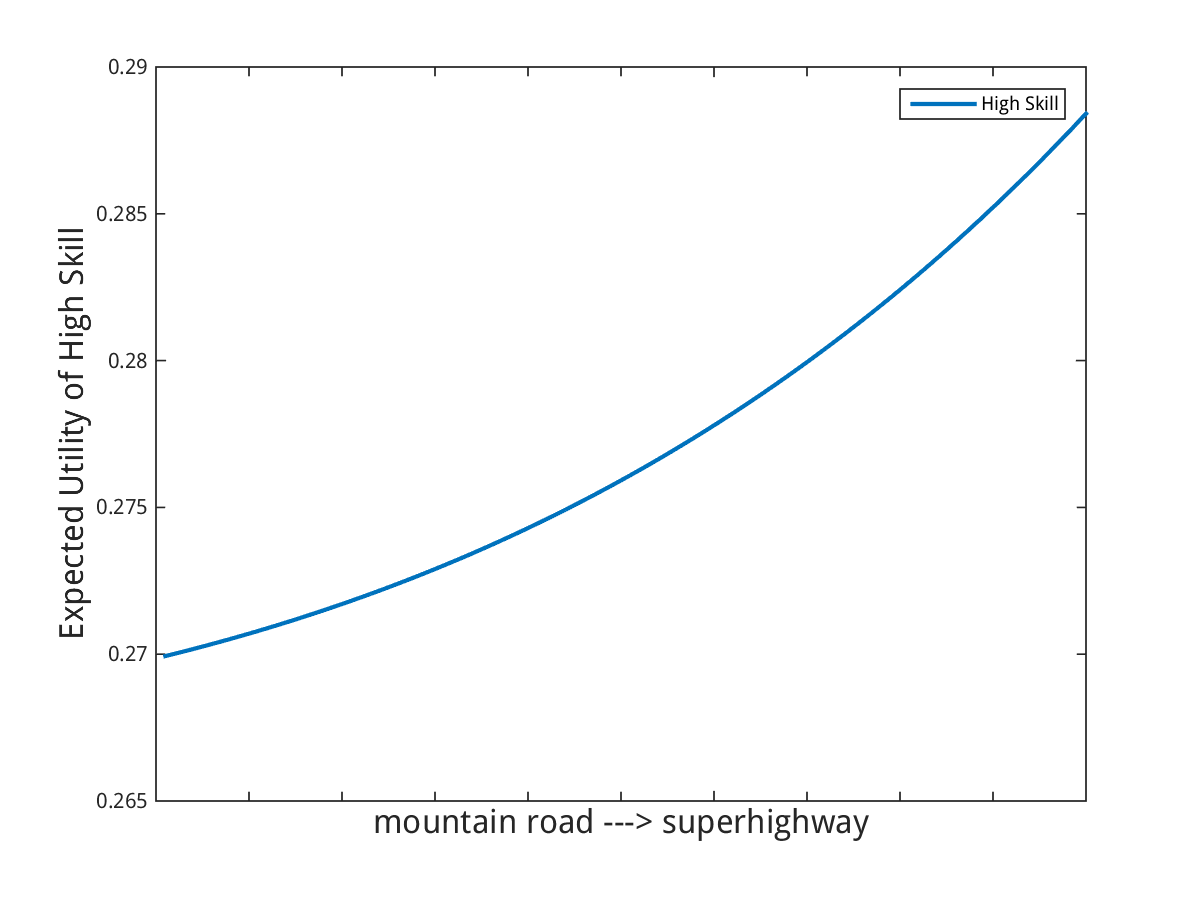
\includegraphics[width=0.5\textwidth]{pics/mr_welfarehigh.png}}
\subfloat[Unskilled welfare]{
\label{fig:abs_wel_unskilled}
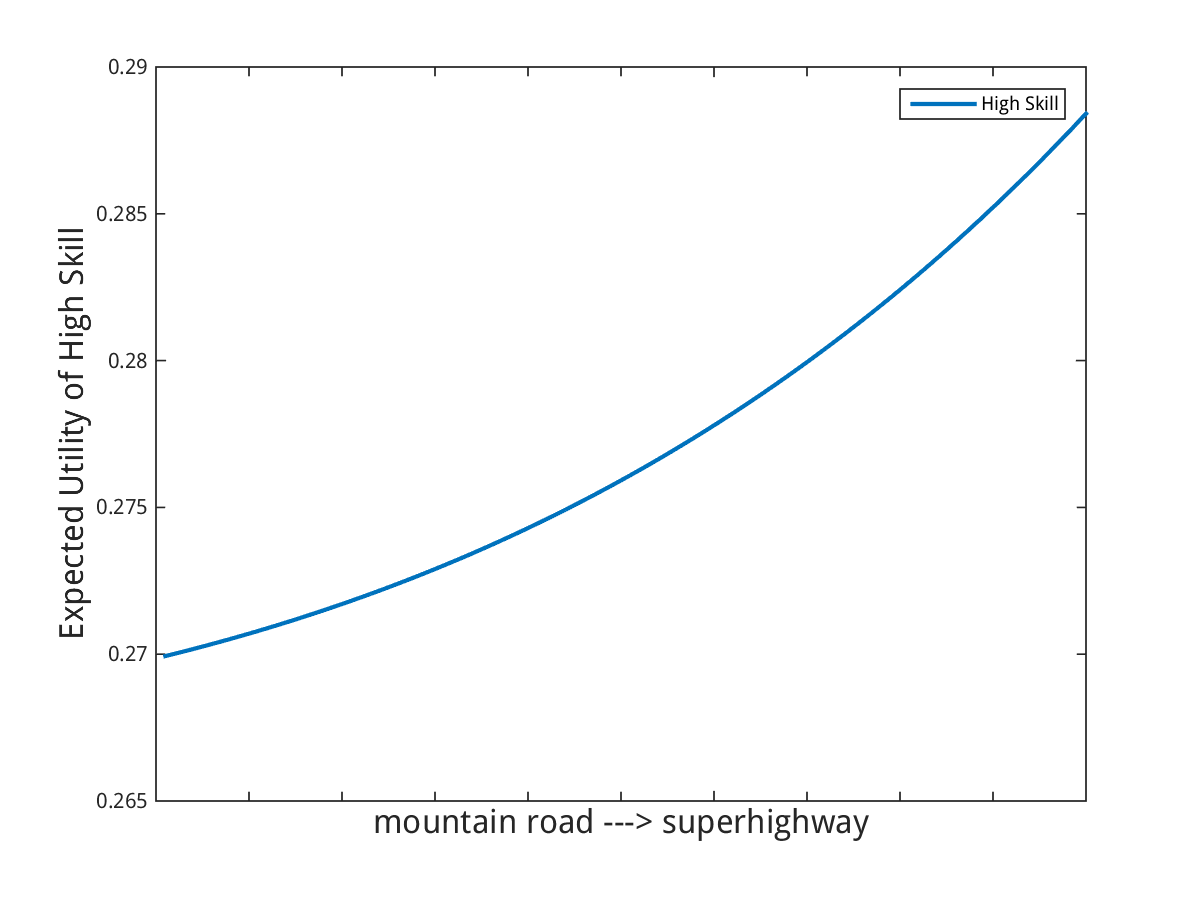
\includegraphics[width=0.5\textwidth]{pics/mr_welfarehigh.png}}

\subfloat[Total population]{
\label{fig:pop_shr}
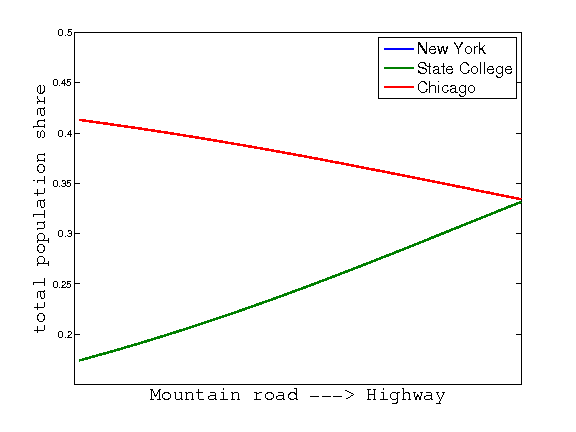
\includegraphics[width=0.5\textwidth]{pics/mr_populationshare.png}}
\subfloat[Skilled population share]{
\label{fig:skl_shr}
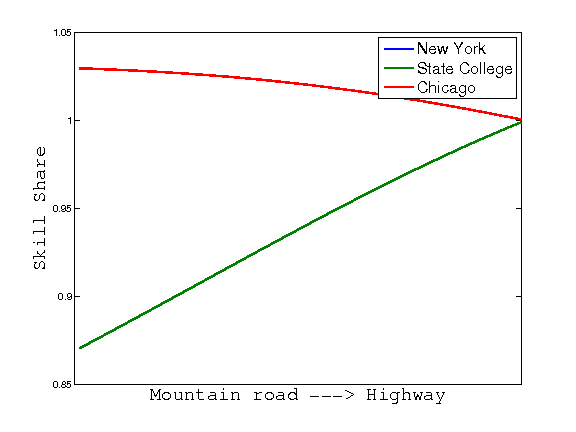
\includegraphics[width=0.5\textwidth]{pics/mr_skillshare.png}}

\subfloat[Skilled wage premium]{
\label{fig:skl_prm}
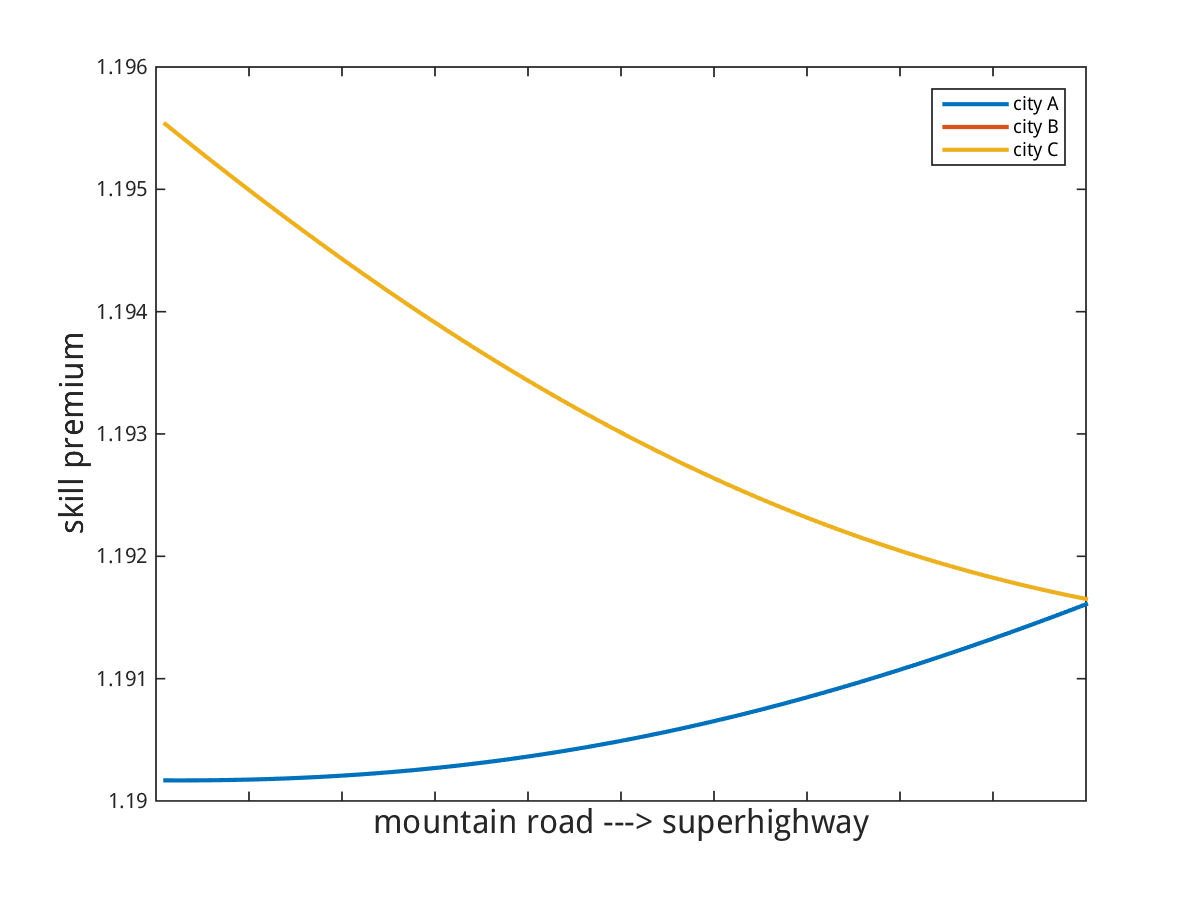
\includegraphics[width=0.5\textwidth]{pics/mr_skillpremium.png}}
\subfloat[Relative welfare (skilled to unskilled)]{
\label{fig:rel_wel}
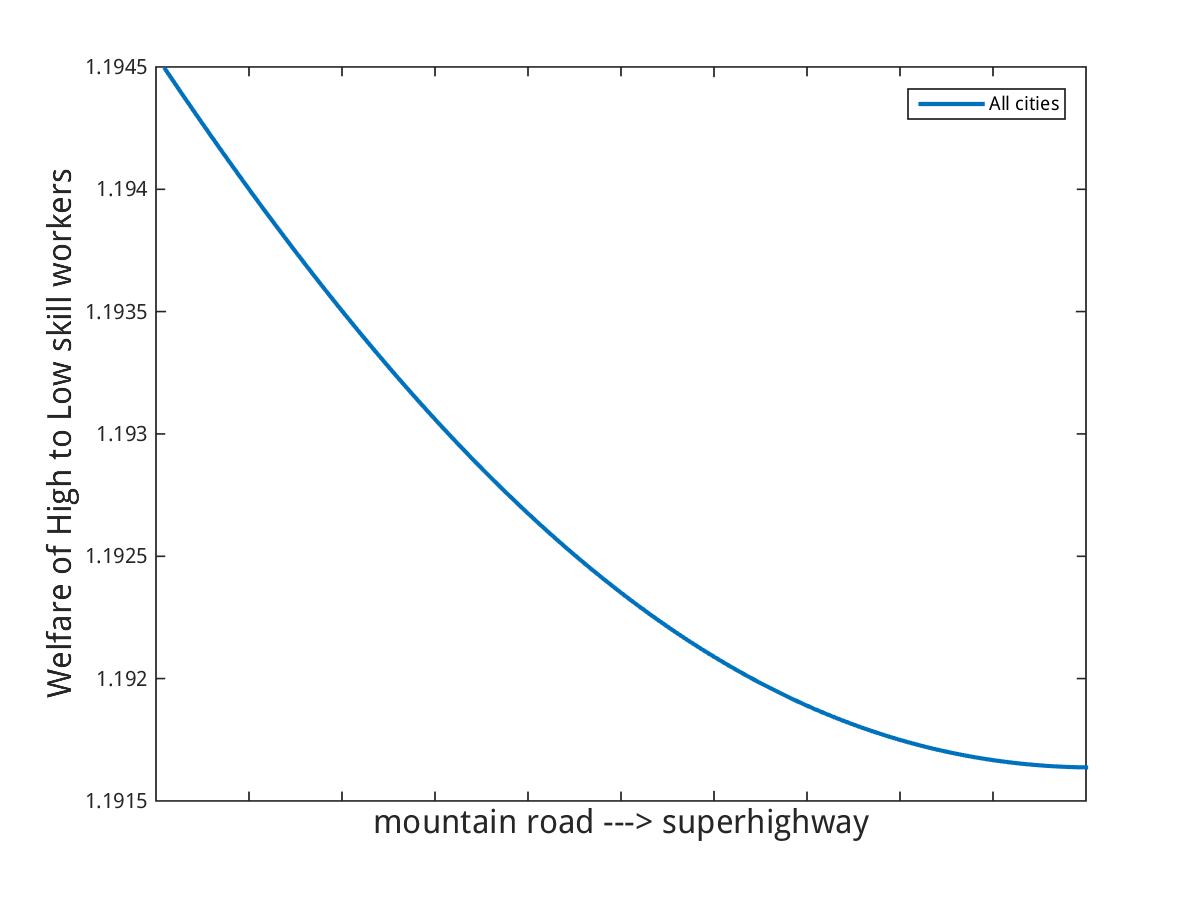
\includegraphics[width=0.5\textwidth]{pics/mr_welfareH2L.png}}

\centering
\caption{\label{fig:sim_res} Reducing cost of reaching State College}
\end{figure}

\section{Conclusion}

We find that remote cities have both a relatively low college wage premium, and a relatively low college educated population share.  This result holds even after controlling for city size.  The stylized facts motivate our development of a spatial equilibrium model.  We show that both heterogenous location preferences among workers and stronger agglomeration forces for skilled workers deliver the moments we find in the data.  In simulations, we find that the model works as expected, and find that reducing the costs of trade benefits unskilled workers more than skilled workers.

While our model delivers simple intuition, it is rich enough to estimate using American data.  We are currently in the process of estimating the model.  Once the model is estimated, we will run counterfactuals relating trade costs to changes in the distribution of nominal and real wage inequality.  These results will be added to this working paper when they are available.

% \begin{figure}[!ht]
% \centering
% \subfloat[high skill util]{ 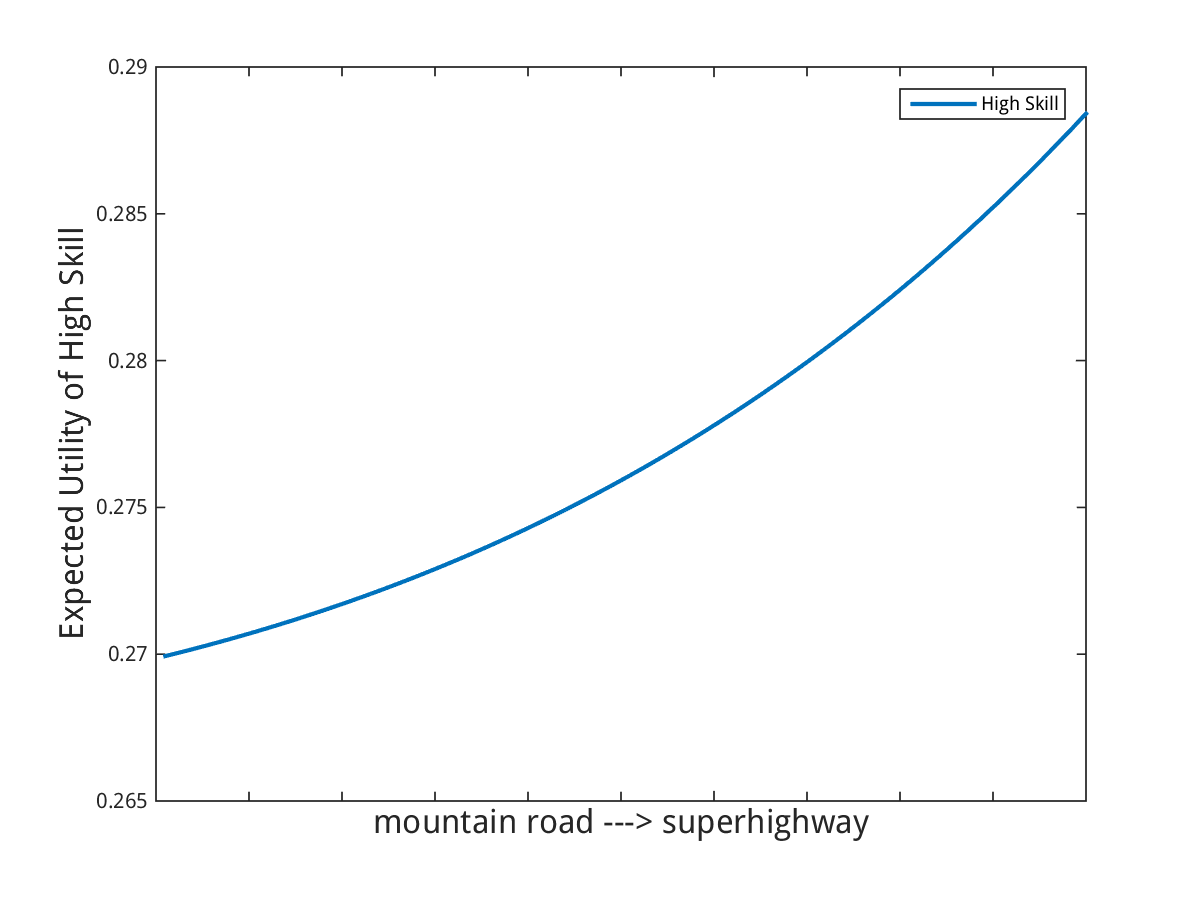
\includegraphics[scale=.35]{pics/mr_welfarehigh.png}}
% \subfloat[low skill util]{ 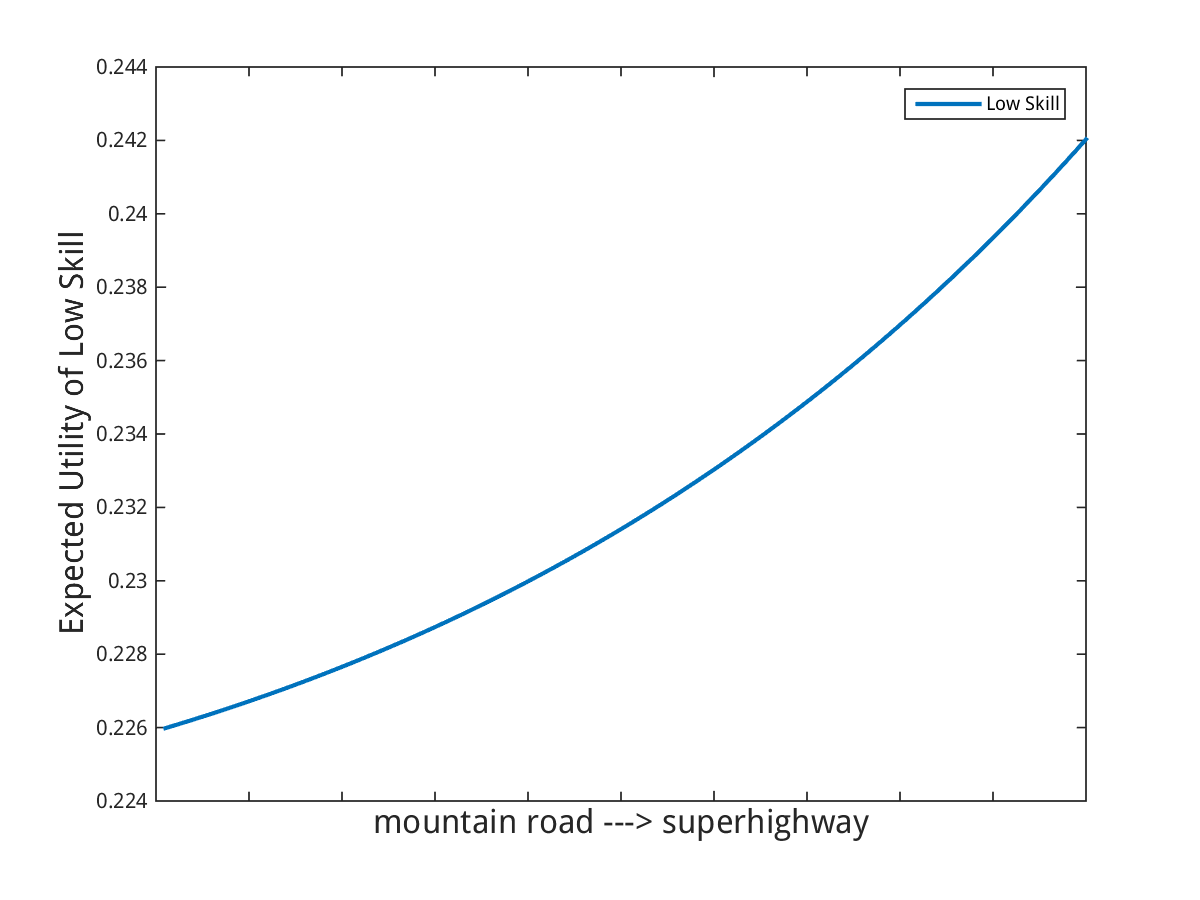
\includegraphics[scale=.35]{pics/mr_welfarelow.png}}
% \caption{Welfare changes by skill type}
% \label{fig:abs_wel}
% \end{figure}
% 
% \begin{figure}[!ht]
% \centering
% 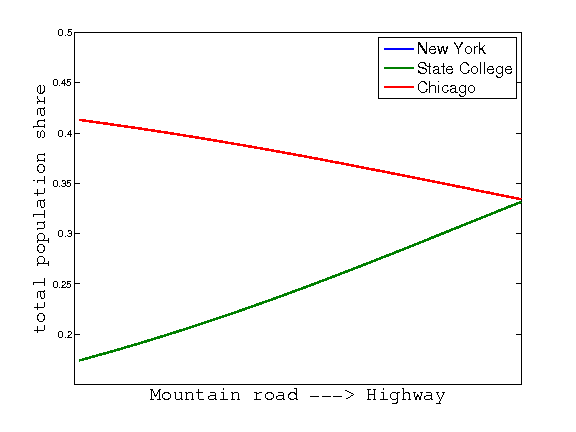
\includegraphics[scale=.4]{pics/mr_populationshare.png}
% \label{fig:pop_shr}
% \caption{Total population share}
% \end{figure}
% 
% \begin{figure}[!ht]
% \centering
% 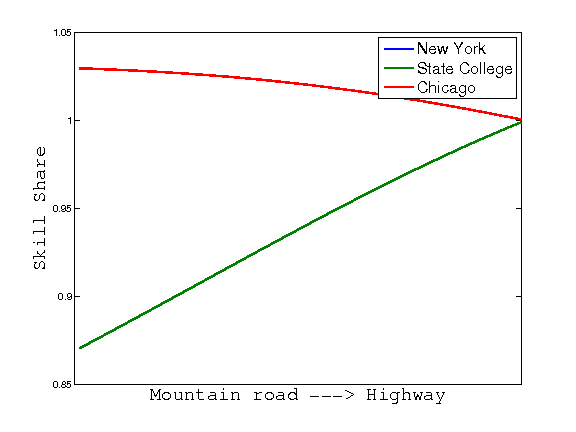
\includegraphics[scale=.4]{pics/mr_skillshare.png}
% \label{fig:skl_shr}
% \caption{Skilled population share}
% \end{figure}
% 
% \begin{figure}[!ht]
% \centering
% 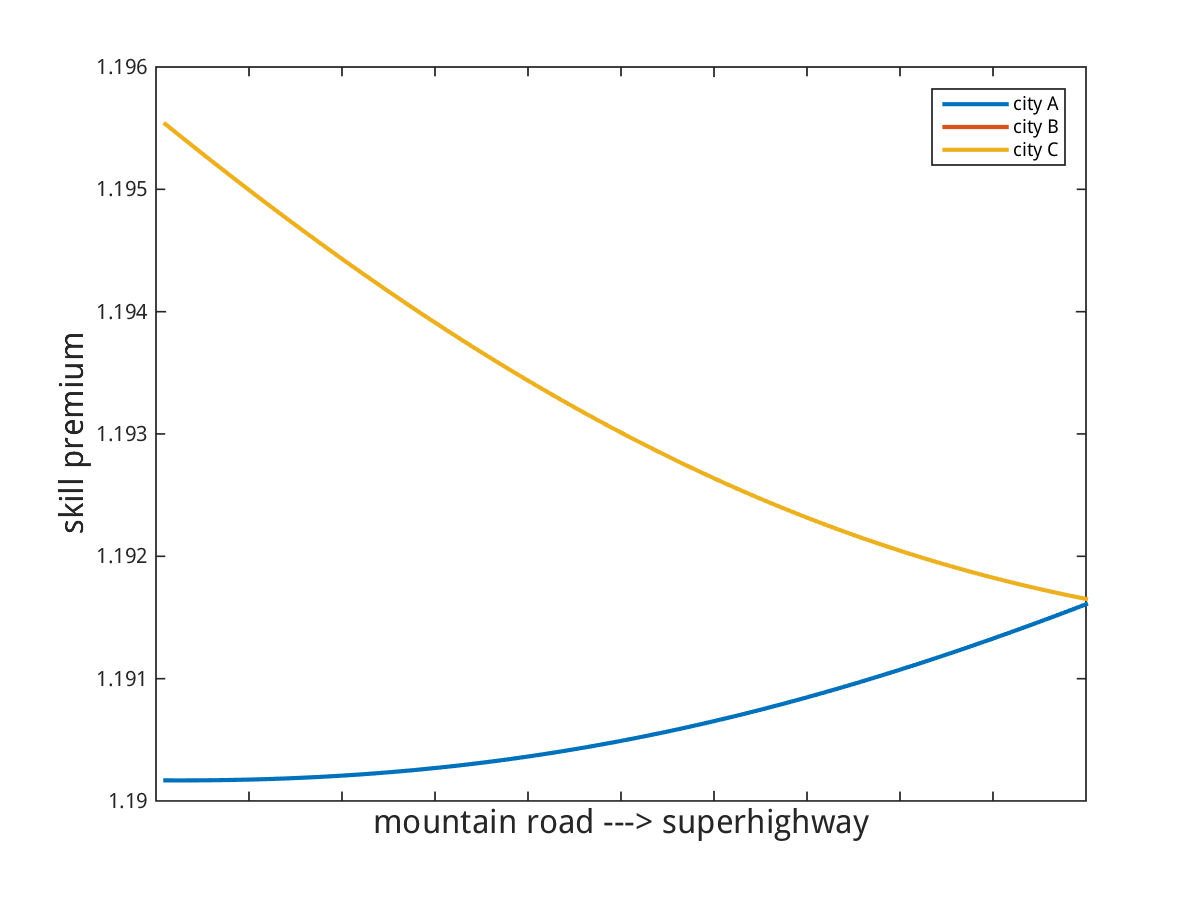
\includegraphics[scale=.4]{pics/mr_skillpremium.png}
% \label{fig:skl_prm}
% \caption{Skilled wage premium}
% \end{figure}
% 
% \begin{figure}[!ht]
% \centering
% 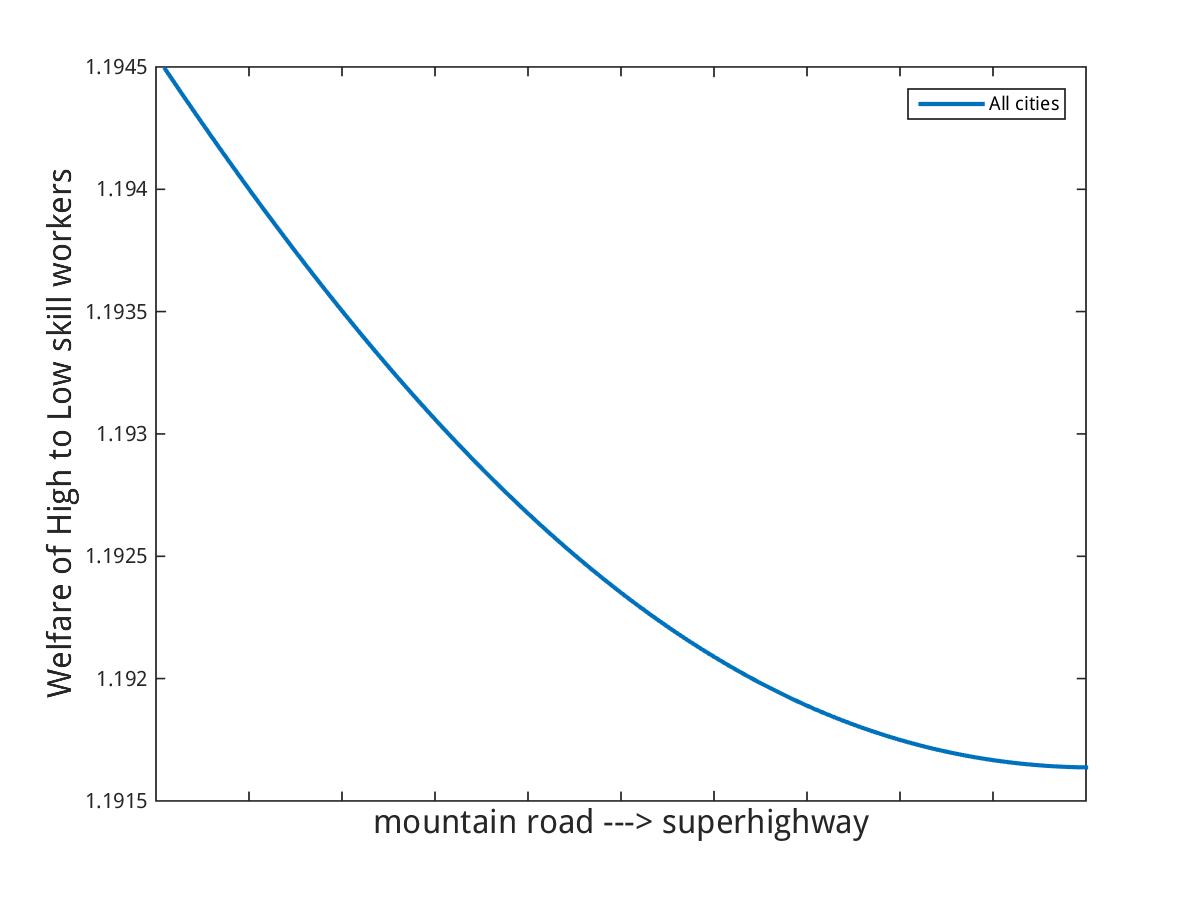
\includegraphics[scale = 0.4]{pics/mr_welfareH2L.png}
% \label{fig:rel_wel}
% \caption{Relative welfare change, skilled over unskilled}
% \end{figure}

\newpage

\bibliographystyle{apa.bst}
\bibliography{/home/veryshuai/Documents/bib/biglist}

\appendix
\section{Solution Algorithm}
\label{sec:sol_alg}

\begin{enumerate}
\item Guess $n_H(i)$ for all $i$.
\item Compute $W_H/W_L$ according to (\ref{eq:WHtoL}). Then plug it in (\ref{eq:labor_demand_supply_2}) to find $n_L(i)$.
\item Calculate skill premia, $\omega(i) \equiv w_H(i)/w_L(i)$, according to (\ref{eq:labor_demand_supply}).
\item Compute $b(i)
= 1/(1 + \frac{n_L(i)}{n_H(i)} \frac{1}{\omega(i)})$
\item Find $\tilde{c}(i)$ according to (\ref{eq:ctilde}).
\item Calculate $w_H(i)$ according to (\ref{eq:systems_relation}) up to scale parameter $\lambda$,
\[
w_H(i) \equiv \lambda^{\frac{1}{2\sigma-1}} \tilde{w}_H(i)
\]
where
\[
\tilde{w}_H(i) = b(i)^{\frac{1}{2\sigma-1}} A(i)^{\frac{\sigma-1}{2\sigma-1}}\tilde{c}(i)^{\frac{1-\sigma}{2\sigma-1}} u(i)^{\frac{1-\sigma}{2\sigma-1}} n_H(i)^{\frac{\sigma-1-\theta}{\theta(2\sigma-1)}}
\]
\item Let $f(i)=\tilde{w}_H(i)^{1-\sigma}$, $\kappa=W_H^{1-\sigma} N_H^{\frac{\sigma-1}{\theta}}$, and
\[
K(j,i) = n_H(i)^{(1-\sigma)/\theta}u(i)^{\sigma-1} d(j,i)^{1-\sigma} A(j)^{\sigma-1} \tilde{c}(j)^{1-\sigma}
\]
Then, system of integral equations (\ref{eq:system2}) can be written as follows (note that the scale parameter cancels out):
\[
f(i) = \kappa \int_J K(j,i) f(j)~dj
\]
In iteration $t$, update $f^{(t)}(i)$ according to
\begin{eqnarray}
	f^{(t+1)}(i) = \frac{\int_J K(j,i) f^{(t)}(j)~dj}{\int_J \int_J K(j,i) f^{(t)}(j)~dj di}
\end{eqnarray}
Note that we do not need to know $\kappa$ to update our guess. If $f^{(t+1)}(i)$ is not close enough to $f^{(t)}(i)$, go to step 2. Otherwise, go to the next step. 
\item Find $\lambda$ by $\int_J w_H(j) dj =1$ (the normalization defined in equilibrium),
\[
1=\int_J w_H(j) dj = \int_J f(j)^{\frac{1}{1-\sigma}} dj = \lambda^{\frac{1}{(1-\sigma)(2\sigma-1)}} \int_J \tilde{w}_H(j)^{\frac{1}{1-\sigma}} dj
\]
So,
\[
\lambda = \Big[\int_J \tilde{w}_H(j)^{\frac{1}{1-\sigma}} dj\Big]^{(\sigma-1)(2\sigma-1)}
\]
From here, find $w_H(i)$.
\item Find $\kappa$,
\[
\kappa = \frac{ f(i)} {\int_J K(j,i) f(j)~dj} = \frac{f(\ell)}{\int_J K(j,\ell) f(j)~dj} 
\]
The above should hold for all $i$ and $\ell$. This step, thus, is also a check that the solutions to integral equations are correct. Then, calculate: 
\[
W_H = N_H^{\frac{1}{\theta}}\kappa^{\frac{1}{1-\sigma}}
\]
Once $w_H(i)$ and $W_H$ are known, it is straightforward to calculate all other equilibrium objects.
\end{enumerate}
\end{document}
